
\begin{figure}[b]
\centering
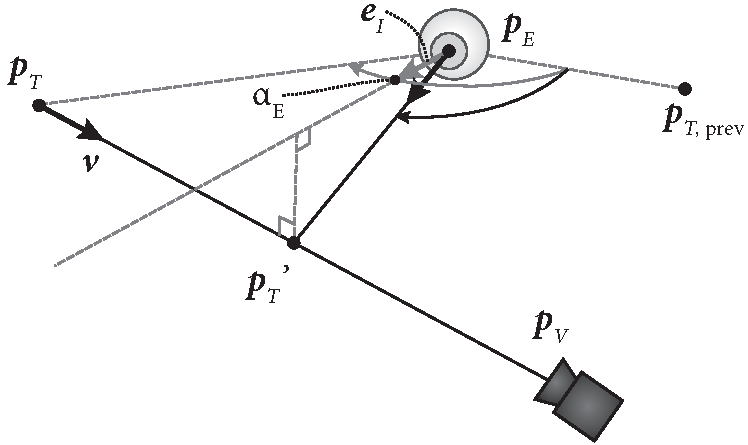
\includegraphics[width=0.5\textwidth]{Figures/EyeAlignment.pdf}
\caption{Computing effective gaze target position in a performative gaze shift.}
\label{fig:EyeAlignment}
\end{figure}

\begin{figure}
\centering
\includegraphics[width=0.48\textwidth]{Figures/PerformativeGazeExample.pdf}
\caption{Examples of performative gaze shifts.}
\label{fig:PerformativeGazeExample}
\end{figure}

While normal human gaze has the primary function of enabling the person to look at a particular object, in acting and cartoon animation the primary purpose of gaze is to communicate ideas to, and create engagement with the audience. This is often achieved by performing partial gaze shifts in general direction of the object, to convey the idea that the character is looking at the object, without actually establishing eye contact with it. That way the character retains partial alignment with the audience, which is known to have a number of benefits in social interaction. For example, in the context of virtual characters, a recent study \cite{andrist2012designing} has shown that the character is seen as more likable, trustworthy, and engaging when it maintains more head alignment with the viewer.

Our model provides explicit support for partial gaze shifts, by exposing the eye alignment parameter $\alpha_E$, which allows the designer to specify the desired amount of alignment with the target. The character will then gaze at a point directly between the gaze target and the viewer; we call this point the \textit{effective gaze target}. In order to "trick" the viewer into accepting that the character is gazing at the real target, the two targets must occupy the same position in the screen space.

%The justification for this relaxation of a fundamental functional constraint of gaze comes from prior research, which indicates that humans are poor at judging the gaze direction of other humans, unless the latter are gazing directly at them. Studies done by Von Cranach et al. \cite{cranach1973looking} indicate that observers have a better than random chance of identifying face-directed gaze at very low viewing angles, but beyond that they rely more on head orientation to estimate gaze direction. That is also why our eye alignment technique, much like the target pose adaptation techniques from the previous section, must be applied in a view-dependent manner -- we allow more deviation from original target pose at greater target viewing angles.
% Does this actually provide support for eye alignment technique? After all, this technique alters target head orientation as well, which directly violates Von Cranach's principle that humans rely on head orientation to judge gaze direction. I still think this belongs in the target pose adaptation section, moreso since I consulted Von Cranach's study when designing those (and only those) techniques.

Figure~\ref{fig:EyeAlignment} illustrates how correct partial eye alignment is achieved. We compute the intermediate rotation of each eye $E$ as $q_I = slerp ( q_S, q_T, \alpha_E )$, where $q_S$ and $q_T$ are eye rotations in the source and target pose, respectively. At this rotation, the eye's gaze direction is given by vector $\mathbf{e_I}$. The view direction $\mathbf{v}$ points from the target $T$ to the viewer; we compute the point on $\mathbf{v}$ that is closest to $\mathbf{e_I}$. This point, $\mathbf{T'}$, is the effective gaze target position.

Like our target pose adaptation techniques (Section~\ref{sec:TargetPoseAdaptation}), eye alignment is applied in a view-dependent manner. For low values of the target viewing angle $\phi_T$ we must enforce full or nearly-full eye alignment, otherwise the viewer might notice the character is not actually gazing at them. Designer-specified eye alignment must therefore be adjusted by the viewing cone parameter $p_{\phi}$, as follows:

\begin{equation}
\alpha_E' = 1 - p_{\phi} + \alpha_E p_{\phi}
\end{equation}

Examples of performative gaze can be seen in Figure~\ref{fig:PerformativeGazeExample}. In both examples, the character is gazing at the red sphere to their right. However, while in the left image the character's eyes are fully aligned with the sphere, in the right image the alignment is established only in screen space; the character cannot actually see the sphere, even if it appears to be gazing at it.
